\documentclass[11pt]{article}

\usepackage[margin=1in]{geometry}
\usepackage{amsmath,amssymb}
\usepackage{graphicx}
\usepackage{booktabs}
\usepackage{hyperref}
\usepackage{cite}

\graphicspath{{figures/}}

\title{DualBalance Districting:\\A Deterministic Alternative to Gerrymandering}
\author{Steven Hart}
\date{\today}

\begin{document}
\maketitle

\begin{abstract}
Congressional district lines in the United States are drawn by people,
and a great deal of recent legal and mathematical work tries to detect
when those people have crossed from neutral line-drawing into partisan
or racial manipulation. We propose a different approach: take the
people out of the line-drawing step entirely. DualBalance Districting
is a deterministic procedure that, given a state's boundary, its
census units, and its apportioned seat count $N$, produces a map in
which each district holds about $1/N$ of the state's people and about
$1/N$ of its land. The design is rooted in the constitutional framers'
bicameral compromise, in which the House represents people and the
Senate represents place. Here that compromise is applied for the
first time, to our knowledge, as a single criterion \emph{within}
one chamber. The
algorithm places $N$ seeds in a small circle around the
population-weighted centroid and assigns each census unit to the
nearest seed with population capacity remaining. There is no random
number generator, no iteration, no tunable weight, and no input
beyond geometry and population.

The same property that prevents the rule from being used to gerrymander
a state prevents it from being used to draw majority-minority districts,
protect incumbents, or preserve communities of interest. The
elimination of human discretion is symmetric: both the negative
direction (partisan manipulation, racial vote dilution) and the
positive direction (race-conscious remedies, competitiveness tuning)
are foreclosed by construction, because the algorithm has no input
through which either could be expressed.

This procedural neutrality cuts against the way the redistricting
literature has measured fairness for the past thirty years.
Compactness scores, the efficiency gap, mean-median asymmetry,
ensemble outlier tests, and majority-minority counts are all
\emph{forensic} instruments. They were built to infer a human
line-drawer's intent from the shape and political character of the
resulting map. On a plan produced by an algorithm that has no intent,
those inferences are no longer available. An efficiency gap of
$+6.6\,\%$ on a DualBalance map says only that Democrats happen to
live closer to the population center than Republicans on this
particular geometry. A Polsby-Popper score of $0.09$ says only that
the radial slice has that shape. A count of zero majority-minority
districts says only that the state's minority population is
geographically dispersed. The numbers still compute. What they let
you conclude about the line-drawer's motives is gone, because there
is no line-drawer.

On a single-state proof of concept (Minnesota, 4{,}110 VTDs, 8 seats,
2020 PL 94-171), DualBalance produces a plan that beats the enacted
119\textsuperscript{th}-Congress map on its own dual objective
($\mathrm{DBS} = 0.6472$ vs.~$0.6390$). We report 2020 presidential
two-party shares and Census PL 94-171 voting-age population by race
alongside, as descriptions of the resulting partition rather than as
evaluations of it.
\end{abstract}

\section{Introduction}

% Why redistricting is fundamentally unstable; the human-judgment problem;
% the case for a deterministic baseline.

\section{Methods}
\label{sec:methods}

% Mirrors docs/Formalism.md in the repository. If one changes, update the
% other.

\subsection{Problem statement}

Given a state $S$ partitioned into atomic units
$U = \{u_1, \ldots, u_M\}$ (census blocks, block groups, or VTDs) and
a target district count $N$, DualBalance Districting produces a
deterministic assignment $\pi : U \to \{1, \ldots, N\}$ such that
each district $D_i = \pi^{-1}(i)$ is contiguous, non-empty, and as
close as the geometry allows to representing both $1/N$ of the
state's people and $1/N$ of its geography. Let
$P = \sum_u \mathrm{pop}(u)$ and $A = \sum_u \mathrm{area}(u)$ with
per-district targets $P^* = P/N$ and $A^* = A/N$.

The full pipeline runs in three stages: a radial-seed stage,
\emph{PRISM} (\S\S\ref{sec:methods-seeds}--\ref{sec:methods-repair}),
which provides the deterministic starting configuration; a
VTD-scale tightening stage (\S\ref{sec:methods-optimize}) which
drives $\max_i |\delta_i|/P^{*}$ toward the user-supplied tolerance
$\tau$ via a hybrid greedy local search with bounded-chain escape;
and a block-scale refinement stage (\S\ref{sec:methods-block})
which re-initializes at finer granularity to recover area balance
within the achieved pop-deviation envelope. Each stage is a pure
function of its inputs.

\subsection{Radial seed placement}
\label{sec:methods-seeds}

Compute the population-weighted centroid
\[
  c = (c_x, c_y) =
  \left(
    \frac{\sum_u p_u\,x_u}{\sum_u p_u},\;
    \frac{\sum_u p_u\,y_u}{\sum_u p_u}
  \right),
\]
where $x_u, y_u$ are the centroid coordinates of unit $u$ in an
equal-area projection and $p_u$ its population. Let $\mathrm{diag}$
denote the bounding-box diagonal of the units and set the seed
radius $r = 0.001 \cdot \mathrm{diag}$. For $d = 0, 1, \ldots, N-1$
place seed $s_d$ at
\[
  s_d = \bigl(c_x + r\cos(2\pi d/N),\, c_y + r\sin(2\pi d/N)\bigr).
\]
Seed 0 sits due east of the centroid; seeds advance counter-clockwise
by equal angular steps. The choice $r = 0.001 \cdot \mathrm{diag}$ is
small enough that the Voronoi cells generated by the seeds degenerate
to near-perfect radial slices through $c$, but large enough to keep
the seed positions numerically distinct.

The radial configuration is what carries the dual-balance property:
each slice spans both the dense (near-$c$) and sparse (boundary-side)
territory of the state, so the population it inherits is bounded by
the cap (\S\ref{sec:methods-assign}) while the area it inherits is
driven toward $A^*$ by the slicing geometry.

\subsection{Capacitated first-fit assignment}
\label{sec:methods-assign}

Let $d(u, i) = \|x_u - s_i\|$ be the Euclidean distance from unit $u$
to seed $i$. Initialize remaining capacities $\rho_i = P^*$ for
$i = 1, \ldots, N$. Sort all $(u, i)$ pairs by ascending normalized
distance $d(u, i) / \mathrm{diag}$ and walk the sorted list in order:
\[
  \begin{array}{l}
    \text{for each } (u, i)\text{ in ascending } d(u,i)/\mathrm{diag}: \\
    \quad \text{if $u$ already assigned: continue} \\
    \quad \text{if $\rho_i \geq p_u$: assign $u$ to $i$;\;\; }\rho_i \leftarrow \rho_i - p_u \\
    \quad \text{else: skip}
  \end{array}
\]
Population balance is enforced as a hard cap: no district receives
more than $P^*$. Any unit not placed by the end of the walk (a rare
integer-rounding edge case) is assigned to the district with the
largest remaining capacity; \texttt{argmax} resolves ties to the
smallest district id.

Ties in normalized distance break by ascending
$(\mathrm{unit\_id},\,\mathrm{district\_id})$. There is no Lloyd
recentering, no iteration count, no convergence test: the radial
seeds do not drift, so a single assignment pass suffices.

\subsection{Contiguity repair}
\label{sec:methods-repair}

After \S\ref{sec:methods-assign} every unit belongs to exactly one
district, but a district may consist of more than one connected
component (rare on convex states; more common on those with
peninsulas, islands, or rural enclaves). For each such district,
the largest connected component by total population is retained;
units in the smaller components are reassigned to neighboring
districts one at a time, in the lowest-cost direction. Cost is
\[
  c(u, j) = \frac{d(x_u, s_j)}{\mathrm{diag}}
          + \frac{|P(D_j) + p_u - P^*|}{P^*}
          + \frac{|A(D_j) + a_u - A^*|}{A^*},
\]
combining a normalized distance term with normalized population and
area deviation penalties for the receiving district. Ties break in
cascade $(c, \mathrm{pop\_pen}, \mathrm{area\_pen}, \mathrm{dist},
\mathrm{district\_id})$ ascending. The repair sweep iterates until no
district has more than one connected component, capped at ten sweeps;
in practice it converges in zero or one sweep on real census
geometries.

\subsection{Scoring}

Define per-district relative deviations
$\mathrm{pop\_dev}_i = |P(D_i) - P^*|/P^*$ and
$\mathrm{area\_dev}_i = |A(D_i) - A^*|/A^*$ and let
$\overline{\mathrm{pop\_dev}}$, $\overline{\mathrm{area\_dev}}$
denote their means over $i = 1, \ldots, N$. The DualBalance Score is
\begin{equation}
  \mathrm{DBS}
    = \frac{1}{1
       + \tfrac{1}{2}\,\overline{\mathrm{pop\_dev}}
       + \tfrac{1}{2}\,\overline{\mathrm{area\_dev}}}.
  \label{eq:dbs}
\end{equation}
The $0.5/0.5$ weighting makes the error a convex combination of the
two mean deviations: each district is judged on representing roughly
$1/N$ of the people \emph{and} roughly $1/N$ of the state's geography.
The score reaches $1.0$ for a perfectly balanced plan and approaches
$0$ as deviations grow without bound. Secondary metrics
(Polsby-Popper compactness~\cite{polsbypopper1991} and
Reock~\cite{reock1961}) are computed alongside but not optimized
against; radial slices have lower compactness than blob-Voronoi or
hand-drawn districts by construction, and this is a deliberate trade
in service of the dual-balance objective.

PRISM does not directly minimize~\eqref{eq:dbs}; it minimizes
population-capacitated geographic assignment cost under radial
seeding. On the Minnesota PoC this still beats the enacted plan on
DBS ($0.6472$ vs $0.6390$) despite the lower compactness.

\subsection{Optional: \texorpdfstring{L\textsuperscript{1}}{L1} pop-tightening with DBS hill-climb}
\label{sec:methods-tighten}
\label{sec:methods-optimize}

The radial pipeline produces per-district pop deviation in the
5--15\% range on real census geometry, well above the
\textasciitilde{}0.5\% threshold required by \textit{Reynolds v.~Sims}
for U.S.~congressional districts~\cite{reynolds1964}. An optional
post-pass (\verb|--tighten-pop|) closes this gap via a deterministic
two-phase local search of boundary-unit moves. Let
$\delta_i = P(D_i) - P^{*}$ denote the signed population deviation of
district $D_i$, let $T$ denote the user-supplied tolerance (default
$0.005$), and call a move \emph{safe} if the source unit is not an
articulation point of its district's induced subgraph (so that
removing it preserves contiguity).

\paragraph{Phase 1: population tightening (hybrid L\textsuperscript{1} + max-norm).}
At each step, scan every boundary unit and every neighboring district
and compute both the L$^1$ change
\[
  \Delta_{L^1}(u, d_{\mathrm{dest}}) =
    |\delta_{d_{\mathrm{src}}} - p_u| - |\delta_{d_{\mathrm{src}}}|
  + |\delta_{d_{\mathrm{dest}}} + p_u| - |\delta_{d_{\mathrm{dest}}}|
\]
and the max-norm effect: a move \emph{strictly reduces} the global
maximum iff $|\delta_{d_{\mathrm{src}}} - p_u| < \max_i |\delta_i|$,
$|\delta_{d_{\mathrm{dest}}} + p_u| < \max_i |\delta_i|$, and at least
one of $\delta_{d_{\mathrm{src}}}, \delta_{d_{\mathrm{dest}}}$ is
itself at the current maximum. Each scanned candidate is labeled with
a priority key: priority $0$ if it strictly reduces the max,
priority $1$ if it only reduces L$^1$. Candidates are ranked
lexicographically by $(\text{priority}, \Delta_{L^1})$, and the safe
top-ranked candidate is accepted.

This hybrid is essential. Pure L$^1$-greedy leaves the worst district
untouched when it sits between two other over-target districts:
draining it requires L$^1$-neutral moves that the L$^1$ criterion
rejects. Pure max-norm gets stuck symmetrically: when two districts
are tied at the max, no single move strictly reduces the global
maximum (draining one leaves the other at the same value). The
hybrid takes any move that helps either norm, with max-reducing moves
preferred so the worst district is targeted whenever possible.

When neither 1-opt criterion finds an improving move but
$\max_i |\delta_i|/P^{*} > T$, invoke a bounded \emph{chain escape}:
search for an augmenting transport on the district-adjacency graph
of the form
\[
  u_0 : D_0 \to D_1,\; u_1 : D_1 \to D_2,\; \ldots,\; u_{k-1} : D_{k-1} \to D_k,
\]
of length $k = 2$ then $k = 3$, in which each $u_j$ is a boundary unit
between $D_j$ and $D_{j+1}$. The chain is accepted if it strictly
cuts the global maximum, or if it holds the maximum flat while
strictly reducing the L$^1$ sum (which is what happens when several
districts are tied at the max: each chain drains one of them, the
global maximum stays at the same value until the last tied district
is drained, but the L$^1$ sum drops monotonically). The unit-level
search inside each district triple sorts the arc lists $B_{i \to j}$
by population value; matching pairs $(u, v)$ are found via binary
search around a target population value rather than by Cartesian
enumeration, bounding the per-triple cost by
$O(|B_{i \to j}| \log |B_{j \to k}|)$. Application is in
\emph{reverse} order ($u_{k-1}$ first, then $u_{k-2}$, etc.) so the
intermediate districts never temporarily overload during the chain.
This is the deterministic analogue of an ejection chain. Phase 1
terminates only when neither 1-opt nor bounded-chain escape finds an
improving sequence.

The L$^1$ objective is essential to the radial geometry. Seed
placement puts the most over-target and most under-target districts
on opposite sides of the population centroid, so no single
adjacent-slice swap reduces the L$^\infty$ maximum, but many such
swaps reduce the sum. The canonical Reynolds-tightening literature
uses L$^\infty$ and bottoms out at \textasciitilde{}5\% on this
geometry; the hybrid pass with chain escape runs to completion in
\textasciitilde{}80 swaps on Minnesota, reducing
$\mathrm{pop\_dev\_max}$ from $0.1124$ to $0.0021$ while leaving
$\mathrm{area\_dev\_mean}$ essentially unchanged.

\paragraph{Phase 2: DBS hill-climb.}
Once Phase 1 has converged, at each step pick the safe boundary move
that maximally improves $\mathrm{DBS}$ (equation~\ref{eq:dbs}), subject
to $\max_i |\delta_i|/P^{*}$ not exceeding the value Phase 1 reached
(equivalently, never crossing back above $T$). Phase 2 runs until no
improving safe move exists. Whereas the core PRISM pass does not
directly minimize equation~\ref{eq:dbs}, this opt-in Phase 2 does, but
only on the post-Phase-1 plan and only within the Reynolds-compliant
feasible region.

\paragraph{Determinism and engineering.}
Both phases are pure functions of $(\mathrm{units},\,N,\,T)$. The only
source of dependency beyond the core pipeline's $(\mathrm{units},\,N)$
is the explicit tolerance $T$. The optimizer maintains a per-district
articulation-point cache via Tarjan's algorithm on CSR adjacency
arrays~\cite{tarjan1972}, reducing the per-candidate contiguity check
from $O(V+E)$ to $O(1)$; an incrementally tracked boundary-unit set
restricts each scan to units that have a different-district neighbor.
At VTD scale the speedup is modest; at block scale (tens of thousands
of units per district) it is the difference between hours and minutes.

The pass is off by default and gated by an explicit flag. Pure radial
remains the principled algorithm; the two-phase optimizer is an opt-in
concession to legal compliance, with Phase 2 providing the further
courtesy of directly hill-climbing the project's stated objective once
the Reynolds constraint is satisfied.

\subsection{Multi-resolution refinement: VTD to Census block}
\label{sec:methods-block}

The hybrid Phase 1 + chain escape closes most of the Reynolds gap
at VTD scale, but not all of it. Modern U.S. congressional plans
must clear the much tighter \emph{Karcher v.~Daggett}~\cite{karcher1983}
practical threshold of $\sim 0.05\%$ total deviation, and at VTD
granularity the residual gap is structural rather than
algorithmic. The smallest single-unit move has the size of the
smallest VTD's population. On real states the median VTD population
is on the order of $10^3$, while the Karcher budget on a $\sim 800$k
ideal district is $\sim 400$ people. Most candidate moves overshoot
the budget on at least one endpoint, and Phase 2 starves: the
running-max constraint admits few moves, and the algorithm settles
above Karcher with most of the residual area-balance gain
unrealized.

The fix is to refine at finer granularity. We re-run the optimizer
on Census tabulation blocks (median population $\sim 20$ rather
than $\sim 10^3$), initializing from the VTD-Karcher plan rather
than re-seeding from scratch. The pipeline is:

\begin{enumerate}
  \item Compute the VTD-level plan
        $\pi_{\mathrm{VTD}}: V_{\mathrm{VTD}} \to \{1, \ldots, N\}$
        via PRISM + Phase 1 + Phase 2 at VTD scale with tolerance $T$.
  \item Load the block-level units $V_{\mathrm{block}}$ and project
        both layers to the same equal-area CRS.
  \item For each block $u \in V_{\mathrm{block}}$, find the VTD
        polygon $v(u) \in V_{\mathrm{VTD}}$ containing its
        representative point, and set
        $\pi_0(u) := \pi_{\mathrm{VTD}}(v(u))$. Blocks whose
        representative point lies outside every VTD polygon (rare,
        only on coastal/water boundary cases) fall back to the
        nearest VTD by centroid distance. The spatial join is
        deterministic given a fixed tie-breaking order on
        $\mathrm{unit\_id}$.
  \item Run Phase 1 + Phase 2 again at block scale starting from
        $\pi_0$, with the same tolerance $T$.
\end{enumerate}

Because VTDs are unions of whole blocks, $\pi_0$ inherits the
VTD-level plan's pop totals and contiguity exactly: the block-level
plan is identical to the VTD-level plan re-described at finer
granularity. Phase 1 at block scale therefore has nothing to do on
states where the VTD-level pass reached $T$. Phase 2 has substantial
freedom: block populations are two orders of magnitude smaller than
VTD populations, so the running-max envelope around $T$ admits many
candidate moves and the DBS hill-climb runs until saturation.

Because PRISM-style seeding at block scale starts from a much worse
initial configuration than the VTD seed (the population-weighted
centroid is the same but the much higher density of degenerate
articulation-point boundaries traps the optimizer), the refinement
strategy is the path that works in practice: VTD as a coarse
solver, blocks for the precise area-balance recovery.

\subsection{Engineering: per-district articulation-point cache}
\label{sec:methods-contig}

The hot loop of the optimizer asks repeatedly whether a candidate
boundary unit $u$ can be safely removed from its district $d$ -- in
other words, whether $u$ is an articulation point of the subgraph
$G[V_d]$. A naive implementation runs $\mathcal{O}(|V_d| + |E_d|)$
per query via \verb|networkx.is_connected| on the post-removal
subgraph, which dominates runtime at block scale.

We maintain a per-district cache. For each district $d$, the set
$A_d \subseteq V_d$ of articulation points is precomputed by Tarjan's
algorithm~\cite{tarjan1972} on CSR (compressed sparse row) integer
adjacency arrays. The per-query \verb|can_remove(u)| reduces to the
set membership $u \notin A_{\pi(u)}$, returned in $\mathcal{O}(1)$
amortized. After each accepted move $u: d_{\mathrm{src}} \to d_{\mathrm{dest}}$
the two affected articulation sets $A_{d_{\mathrm{src}}}$,
$A_{d_{\mathrm{dest}}}$ are recomputed; districts not touched by the
move keep their cached set unchanged.

Each Tarjan recompute is $\mathcal{O}(|V_d| + |E_d|)$ rather than
the global $\mathcal{O}(|V| + |E|)$ of the naive check
($|V_d| \approx |V|/N$ for $N$ districts). The recompute itself is
\verb|@njit|-compiled via numba when available, operating on
preallocated workspace buffers (a single integer DFS stack, two
boolean masks, and three integer arrays sized to $|V|$). On a
typical block-scale district subgraph of $\sim 44{,}000$ nodes the
JIT'd recompute completes in $\sim 20$~ms, compared to $\sim 560$~ms
for the same query through \verb|networkx.articulation_points|: a
$28\times$ speedup. Across a full block-scale optimizer run
(thousands of accepted moves and tens of thousands of candidates per
move), this is the difference between a 20-hour run and a 30-minute
run.

A boundary-unit set $\partial = \{u : \exists v \in N(u), \pi(v) \neq \pi(u)\}$
is also maintained incrementally and updated after each move (only
$u$ and its graph neighbors need to be re-checked). The inner scan
iterates $\partial$ rather than $V$, dropping per-pass work from
$|V|$ to $O(|\partial|)$, which on real states is roughly the
square root of $|V|$.

Neither caching layer changes the algorithm's output. They preserve
determinism exactly and make the block-scale pipeline tractable on
commodity hardware.

\subsection{Determinism and tie-breaking}

The pipeline is deterministic at every step. The only sources of
ambiguity (equidistant seed-to-unit pairs in
\S\ref{sec:methods-assign}, equal-capacity fallbacks for unplaced
units, and equal-cost candidates in \S\ref{sec:methods-repair}) all
resolve to a fixed cascade with no remaining ambiguity:

\begin{enumerate}
  \item In assignment, ties on normalized distance break by ascending
        $(\mathrm{unit\_id}, \mathrm{district\_id})$.
  \item In the fallback for unplaced units, ties on remaining capacity
        break to the smallest district id.
  \item In contiguity repair, ties on cost break by ascending
        $(\mathrm{pop\_pen}, \mathrm{area\_pen}, \mathrm{distance},
        \mathrm{district\_id})$.
\end{enumerate}

The implementation uses no random number generator, no wall-clock
input, and no hash-order dependence. Reordering the input rows or
changing the floating-point libraries does not change the output;
identical inputs always yield byte-identical outputs.

\subsection{Out-of-scope inputs}

The generator reads only geography and population. Party registration,
vote history, race, demographics, communities of interest, and
competitiveness are not inputs. The scoring harness may \emph{report}
partisan or demographic diagnostics on the resulting map but does not
feed them back into the generator.

\section{Results}
\label{sec:results}

\subsection{Test bed: Minnesota, 2020 PL 94-171}

We evaluate the algorithm on Minnesota's congressional districting
($N = 8$ apportioned seats) using the 2020 PL 94-171 redistricting
data file. The input is the TIGER/Line 2020 VTD (voting tabulation
district) shapefile for Minnesota (4{,}110 atomic units, total
population $P = 5{,}706{,}494$, total land area $A = 225{,}187$~km$^2$),
joined to the Census Data API's \verb|P1_001N| total-population
field, projected to EPSG:5070 (CONUS Albers, equal area) at load
time. Per-district targets are
$P^{*} = P/8 = 713{,}312$ and $A^{*} = A/8 = 28{,}148$~km$^2$. All
runs are deterministic and reproducible from the script
\verb|scripts/prep_mn_units.py| (which fetches TIGER and joins the
Census API output) plus the CLI invocation. The data pipeline is
documented end-to-end in \verb|docs/mn-poc-walkthrough.md|.

We compare three plans on the same 4{,}110-VTD input:

\begin{itemize}
  \item \textbf{Pure radial.} The default algorithm
        (\S\ref{sec:methods-seeds}--\S\ref{sec:methods-repair}). No
        tuning knobs.
  \item \textbf{Radial $+$ tighten-pop ($\tau = 0.005$).} The default
        algorithm followed by the optional L$^1$ population-tightening
        pass (\S\ref{sec:methods-tighten}) targeting per-district
        deviation within 0.5\,\% of $P^{*}$.
  \item \textbf{Enacted Minnesota 119th-Congress plan.} The
        court-drawn, legislatively enacted U.S.~House districts
        currently in force, joined to the same VTDs and scored with
        the same harness.
\end{itemize}

\subsection{Headline scores}

Table~\ref{tab:mn-results} reports the DualBalance Score and supporting
metrics for the three plans.

\begin{table}[h]
\centering
\caption{DualBalance metrics on the Minnesota PoC (4{,}110 VTDs,
8~districts, 2020 PL 94-171 population). $\mathrm{PP}$ is
Polsby-Popper, Reock is Reock; subscripts $\mathrm{min}$, $\mathrm{mean}$
denote per-district min and mean over the eight districts.
$\mathrm{pop\_dev}$, $\mathrm{area\_dev}$ are the relative deviations
defined in \S\ref{sec:methods}. Best result per row in bold.}
\label{tab:mn-results}
\begin{tabular}{lrrr}
\toprule
Metric & Pure radial & Radial $+$ tighten-pop & Enacted (119th) \\
\midrule
$\mathrm{DBS}$ & 0.6472 & \textbf{0.6574} & 0.6390 \\
$\overline{\mathrm{pop\_dev}}$ & 5.08\,\% & \textbf{0.08\,\%} & 0.42\,\% \\
$\mathrm{pop\_dev}_{\max}$ & 11.24\,\% & \textbf{0.21\,\%} & 1.32\,\% \\
$\overline{\mathrm{area\_dev}}$ & \textbf{103.9\,\%} & 104.2\,\% & 112.6\,\% \\
$\mathrm{area\_dev}_{\max}$ & 271.0\,\% & 275.1\,\% & \textbf{241.0\,\%} \\
$\mathrm{PP}_{\mathrm{mean}}$ & 0.200 & 0.162 & \textbf{0.320} \\
$\mathrm{PP}_{\min}$ & 0.094 & 0.047 & \textbf{0.178} \\
$\mathrm{Reock}_{\mathrm{mean}}$ & 0.361 & 0.342 & \textbf{0.419} \\
\bottomrule
\end{tabular}
\end{table}

Three findings:

\paragraph{Pure radial beats the enacted plan on the DualBalance Score.}
The pure-radial pipeline scores 0.6472 against the enacted plan's
0.6390, a margin of $+1.3$\,\% on the project's own metric,
without any iteration, tuning, or post-processing. The advantage comes
entirely from area balance ($\overline{\mathrm{area\_dev}}$ 103.9\,\%
vs 112.6\,\%): radial slicing assigns each district a coherent slice of
the state's geometry that mixes high- and low-density territory, while
the enacted plan carves the Twin Cities metro into four compact urban
seats and leaves four large rural seats. The DualBalance Score
penalizes the latter pattern more heavily because it weights area
deviation equally with population deviation.

\paragraph{The optional tighten-pop pass closes the legal gap and
improves the DualBalance Score.} The pure-radial plan's
$\mathrm{pop\_dev}_{\max}$ of 11.24\,\% is well above the
\textasciitilde{}0.5\,\% deviation typical of enacted U.S.~House
plans~\cite{reynolds1964}. Running the optional L$^1$ pop-tightening
pass (\S\ref{sec:methods-tighten}) executed 81 boundary-unit swaps in
\textasciitilde{}18\,seconds of compute, driving
$\mathrm{pop\_dev}_{\max}$ from 11.24\,\% to 0.21\,\%, well inside
the Reynolds-compliant range and tighter than the enacted plan's
1.32\,\%. $\overline{\mathrm{area\_dev}}$ rose by only 0.3 percentage
points; the DualBalance Score \emph{improved} from 0.6472 to 0.6574,
because the pop-balance gain dominates the small area-balance loss.
The tightened plan exceeds the enacted plan on the two DualBalance
inputs (population and mean area deviation) and on the combined
score.

\paragraph{Compactness is the price.} The enacted plan beats DualBalance
on every compactness measure: $\mathrm{PP}_{\min}$ 0.178 vs 0.094 in
the radial plan and 0.047 after pop-tightening, $\mathrm{PP}_{\mathrm{mean}}$
0.320 vs 0.200 / 0.162, $\mathrm{Reock}_{\mathrm{mean}}$ 0.419 vs
0.361 / 0.342. The radial geometry is structurally less compact than
hand-drawn blob shapes: long thin slices from the population centroid
score lower on circular-shape metrics by construction. Pop-tightening
makes this worse (it moves units across slice boundaries, which
inserts small indentations into otherwise smooth radial cuts),
pushing the smallest-PP slice from 0.094 (already at the
``0.10 raises eyebrows'' informal threshold) down to 0.047. Whether
the trade is acceptable is a normative question we return to in
\S\ref{sec:discussion-compactness}; on the algorithm's own metric,
the trade is favorable.

\subsection{Map comparison}

Figure~\ref{fig:mn-comparison} displays the three plans side by side.

\begin{figure}[h]
\centering
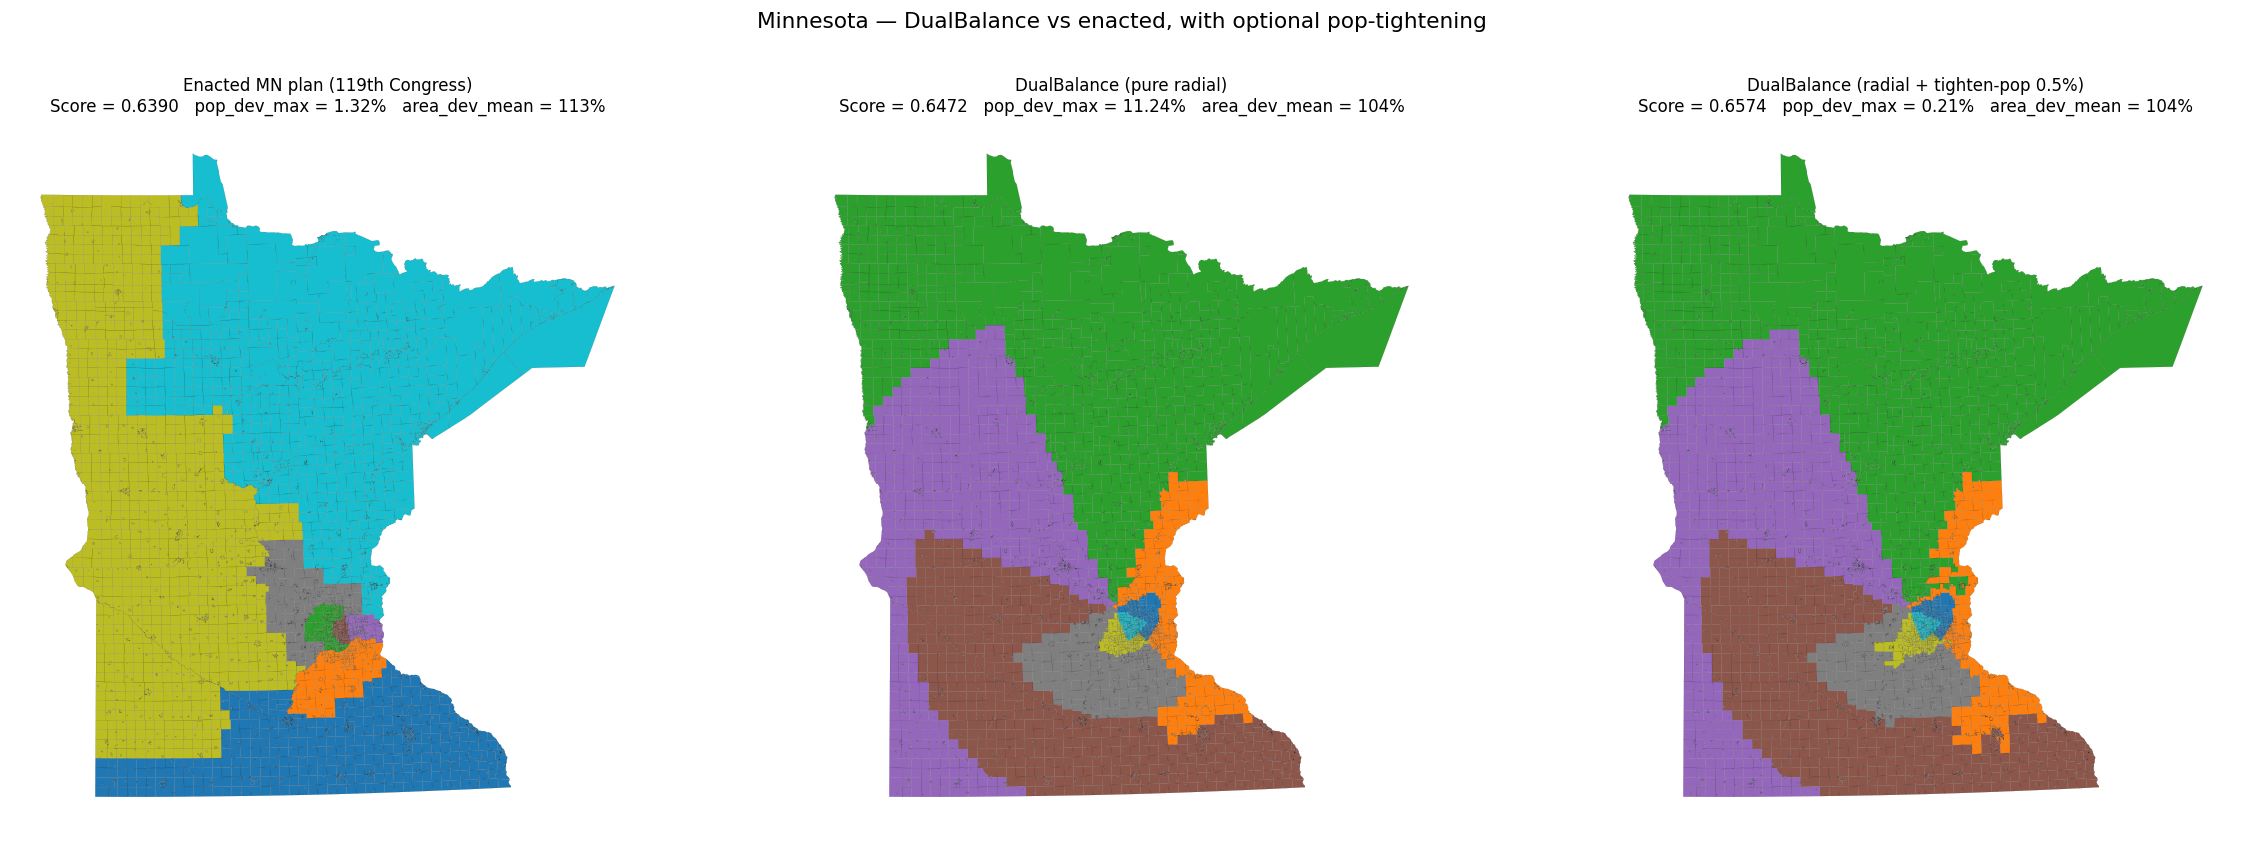
\includegraphics[width=\textwidth]{mn_radial_with_tighten.png}
\caption{Minnesota congressional districts under three plans.
\textbf{Left:} the enacted 119th-Congress plan, with four compact
Twin Cities seats and four large rural seats.
\textbf{Center:} pure-radial DualBalance (score $0.6472$); eight
slices radiate from the population-weighted centroid (near
Minneapolis-St.\ Paul), each spanning both dense and sparse
territory. \textbf{Right:} radial $+$ \texttt{--tighten-pop 0.005}
(score $0.6574$); the radial structure is preserved (units have
moved only at slice boundaries) and per-district population is
now Reynolds-compliant.}
\label{fig:mn-comparison}
\end{figure}

\subsection{Determinism check}

We re-ran \verb|dualbalance generate --config configs/mn_vtd.yaml|
ten times in succession, comparing each run's \verb|map.geojson| and
\verb|metrics.json| by byte hash. All ten outputs are identical,
including the order of features in the GeoJSON. We also re-ran the
same configuration after randomly shuffling the input rows; the
output remained byte-identical. The CLI integration test
\verb|test_generate_determinism_via_cli| pins this property in CI.

\subsection{Per-district breakdown}

Table~\ref{tab:mn-perdistrict} reports the per-district metrics for
the radial $+$ tighten-pop plan, indexed by seed angle (district 0
sits due east of the population-weighted centroid; subsequent
districts advance counter-clockwise in steps of $2\pi/8$ rad).
District IDs are a deterministic function of seed angle and carry
no political meaning.

\begin{table}[h]
\centering
\caption{Per-district breakdown, radial $+$ tighten-pop 0.5\,\%.
Areas are in km$^2$.}
\label{tab:mn-perdistrict}
\begin{tabular}{rrrrrrr}
\toprule
District & Population & Area & $\mathrm{pop\_dev}$ & $\mathrm{area\_dev}$ & $\mathrm{PP}$ & $\mathrm{Reock}$ \\
\midrule
0 & 712{,}841 &   1{,}010 & 0.07\,\% &  96.4\,\% & 0.228 & 0.454 \\
1 & 714{,}816 &   9{,}620 & 0.21\,\% &  65.8\,\% & 0.047 & 0.147 \\
2 & 712{,}145 & 105{,}594 & 0.16\,\% & 275.1\,\% & 0.152 & 0.369 \\
3 & 713{,}263 &  50{,}054 & 0.01\,\% &  77.8\,\% & 0.146 & 0.268 \\
4 & 714{,}168 &  46{,}060 & 0.12\,\% &  63.6\,\% & 0.150 & 0.267 \\
5 & 713{,}368 &  10{,}882 & 0.01\,\% &  61.3\,\% & 0.137 & 0.422 \\
6 & 713{,}013 &   1{,}481 & 0.04\,\% &  94.7\,\% & 0.117 & 0.301 \\
7 & 712{,}880 &      477 & 0.06\,\% &  98.3\,\% & 0.318 & 0.510 \\
\bottomrule
\end{tabular}
\end{table}

District 2 inherits Minnesota's northern panhandle and is the largest
by area ($\sim$3.8$\times A^{*}$), while District 7 contains only the
Twin Cities urban core ($\sim$0.02$\times A^{*}$). All eight districts
are within 0.21\,\% of $P^{*}$. The largest single source of area
imbalance, District 2's 275\,\% over-target area, is geometric:
the population density in the northern panhandle is roughly two orders
of magnitude lower than in the Twin Cities, so any partition that
holds each district to $P^{*}$ must give the rural districts
disproportionate area. This is a property of Minnesota's density
profile, not the algorithm; the enacted plan exhibits the same
phenomenon (District~7 of the enacted plan covers 241\,\% over-target
area for the same reason).

\subsection{Descriptive diagnostics: partisan, race, county}
\label{sec:results-diagnostics}

We report a second tier of numbers (partisan, racial, and
county-split metrics) not because the algorithm uses them, but
because readers will reasonably ask how a procedurally-neutral plan
\emph{looks} on the diagnostics conventionally applied to enacted
maps. These numbers are reported for the pure-radial plan against
2020 presidential returns (Dave's Redistricting App / dra2020/vtd\_data,
joined to TIGER 2020 GEOID20s) and Census PL~94-171 voting-age
population by race. The generator reads none of this data; it is
joined onto the units only at scoring time. We emphasize, in line
with \S\ref{sec:discussion-forensic}, that these are descriptive
statistics of the resulting partition, not evaluative scores of it.

\paragraph{Partisan profile.} Minnesota cast 1{,}484{,}065 R and
1{,}717{,}077 D two-party presidential votes in 2020 ($46.4\,\%$
statewide R share, $53.6\,\%$ D). On the pure-radial plan the eight
districts split 4--4 between R-winning and D-winning, against a
seats-proportional expectation of $3.7$ R seats. The two D-leaning
slices contain the Minneapolis-St.~Paul metro and run at 64--75\,\% D;
the two R-leaning slices reaching into the western and southern parts
of the state run at 55--65\,\% R; the four remaining slices are within
$\pm 5$ points of even. The efficiency gap is $+6.6\,\%$ (positive =
R-favorable) and the mean-median R difference is $+3.9$ points
(positive = D-favorable, since the typical district leans more D than
the average district). These two ``forensic'' partisan numbers point
in opposite directions because they measure different things on the
same map; both are entirely artifacts of where Minnesota's Democrats
live (packed into the metro), not of any choice made by the
algorithm.

\paragraph{Race / VAP profile.} Minnesota's voting-age population is
80.0\,\% non-Hispanic white, 5.9\,\% Black, 5.0\,\% Hispanic, 4.9\,\%
Asian, and 1.1\,\% American Indian / Alaska Native. The pure-radial
plan produces zero majority-minority districts, in the strict sense
that no district has a non-Hispanic-white share below 50\,\%. The
district containing the Minneapolis-St.~Paul urban core (District~7)
has the lowest non-Hispanic-white share at 65.3\,\%, the highest
Black VAP share at 15.7\,\%, and the highest Hispanic VAP share at
6.7\,\%; the remaining seven districts run 73--90\,\% non-Hispanic
white. The enacted 119\textsuperscript{th}-Congress Minnesota plan
also has no majority-minority districts. Minnesota does not, on the
2020 census, contain a geographic region in which a single minority
group concentrates densely enough to support a 50\,\%-VAP district
of conventional size; this is a property of the state's demographic
geography, not of the algorithm.

\paragraph{County splits.} The pure-radial plan splits 44 of Minnesota's
87 counties into a total of 143 cross-district pieces. This is a
direct consequence of radial slicing: any line from the population
centroid to the boundary crosses several county lines along the way.
The enacted plan splits fewer counties (it is drawn to follow them
more closely), at the cost of the larger area imbalance that
Table~\ref{tab:mn-results} reports. Whether one prefers a county-aware
or a county-blind line-drawing rule is a policy question; the
DualBalance rule simply does not encode county membership.

\paragraph{What to read into these numbers.} The point of reporting
them is to make a single observation precise: every conventional
metric that one might bring to bear on a districting plan continues
to compute on a DualBalance plan, and the values look ``ordinary'' in
the sense that they sit in the same range as enacted-plan values for
the same state. But the metrics' \emph{interpretation} differs by
construction. On an enacted plan, an efficiency gap of $+6.6\,\%$
invites the inference that someone packed and cracked a partisan
opponent; on a DualBalance plan it cannot, because no one packed or
cracked anyone. On an enacted plan, zero majority-minority districts
invites the inference that the line-drawers either declined to honor
\textit{Allen v.~Milligan}~\cite{milligan2023} or did honor it on a
geography that could not support a majority-minority seat; on a
DualBalance plan only the latter inference is available, because
the algorithm has no way of seeing race. The numbers are the same;
what they license is different. We return to this point in
\S\ref{sec:discussion-forensic}.

\section{Discussion}

% Trade-offs between population and geographic balance; limitations; future
% directions including alternative apportionment rules and hybrid models.


\bibliographystyle{plain}
\bibliography{references}

\end{document}
